\section{Sourcing Campaigns}
A $^{60}$Co radioactive source, RP4118 with a measured activity of 83.46 $\pm$
0.10 MBq on 14 September 2012, was used to produce the signal readout
during the three sourcing campaigns: HF- in October 2013 with the old PMTs still
installed; HF+ in April 2014 with new PMTs installed; and HF- in July 2014 with
new PMTs installed. First, sourcing with the old PMTs was performed to extract
the source energy deposition in terms of HF calibration durin Run 1. Second, new PMTs were installed and commissioned. Finally, the sourcing was performed with the newly installed hardware and previously extracted source energy deposition was applied to compute the HF gains. Several OVs, which are different from the Voltage that HF is being planned to be operated at during Run II (OV2), were used depending on the histogramming mode (1 TS or 2 TS) as it was important on one hand to take into account the limitations of the QIE range. On the other hand, we have to have sufficient PMT gain not to lose events under the pedestal peak. All HF gains were adjusted for the difference in OVs.

\subsection{2013 HF- Campaign}
Quadrants 1 and 4, also referred to as the near side of HF- containing wedges
1-9, were exposed to the radioactive source on 23 - 27 October 2013, during
which the activity of the source was 72.11 $\pm$ 0.15 MBq. The original
PMTs were used during this campaign in order to obtain the energy deposition
within each tower from the provided radioactive source, as well as to provide
useful data for future studies on radiation damage of the HF calorimeter fibers
precipitating from Run I of the LHC. Data from both quadrants were recorded
with the 1 TS firmware at OV1 (same OV was used during Run I), in
addition to some data recorded with 2 TS firmware at OV1+100. For this
specific campaign the overflow bin must not be included in the analysis
because certain entries are unrelated to the response charge but instead are
indicators of firmware error codes.

Data recording was set to trigger while the radioactive source was within 500 mm
of a source tube. The source driver inserted the radioactive source into a source
tube at a speed of 10 mm/s, held the source at rest approximately 800 mm
from the source tube's back end long enough to collect reasonable statistics
while the source is in the middle of the given tower, and then continued to
insert the source until it reached the back end of the tube. The source is then
immediately retracted from the tube, but in the process the source driver system
must spool the source wire by periodically alternating from retracting to extending the wire to prevent tangles. Overall, approximately 7-8 minutes of data was collected for each source tube, with the majority of the statistics being recorded while the radioactive source was held stationary in the middle of each tower.

To help better illustrate how the data-taking process went and what kind of objects the analysis is performed with, refer to Figure~\ref{fig:hf_campaigns_histograms}. The first graph shows the response of a single channel as source is moving along the source tube inside the tower. Note that source enters from the ''Back'' and moves to the ''Front''. That is because this definition is provided with respect to the CMS Center. Second distribution shows examples of ''signal'' and ''background'' histograms: charge distribution when source is moving inside the tower and another charge distribution when source is moving in some other tower sufficiently isolated from the recorded tower.
\begin{figure}[htb]
    \begin{center}
        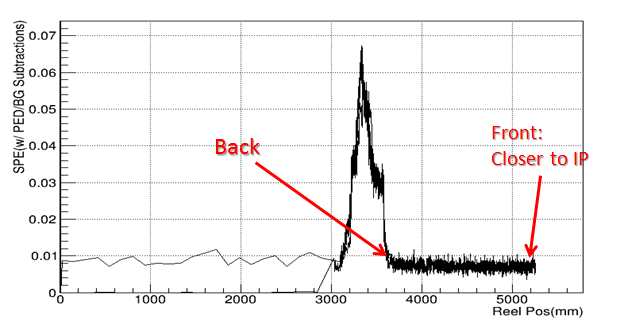
\includegraphics[width=.8\textwidth]{figures/ch_hfcalibration/Signal_ReelPos.png}
        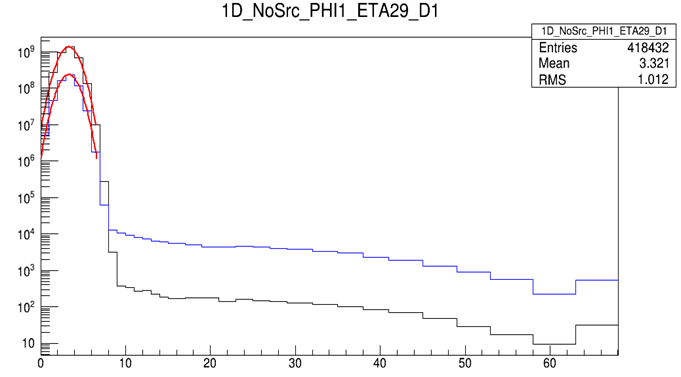
\includegraphics[width=.8\textwidth]{figures/ch_hfcalibration/Signal_Histogram.png}
        \caption
        {(a)Source Signal vs Position (b) 32-bin histogram - A basic object of the read out per a given channel}
        \label{fig:hf_campaigns_histograms}
    \end{center}
\end{figure}

% Run numbers for data collected during this campaign are
% listed in Table~\ref{tab:2013HFM_Runs}.

% \begin{table}[htb] \centering \scalebox{1.10}{
%   \begin{tabular}{|c|c|c|c|c|}
%   \hline
%   Date & Run Number & IPhi & Tubes Sourced & Comments \\
%   \hline
%   \hline
%   23 Oct. & 215590 & 55 & 1A & \\
%   \hline
%   23 Oct. & 215594 & 55 & 1B & \\
%   \hline
%   23 Oct. & 215595 & 55 & 2A-2B & \\
%   \hline
%   23 Oct. & 215596 & 55 & 3A-3B & \\
%   \hline
%   23 Oct. & 215597 & 55 & 4-5 & \\
%   \hline
%   23 Oct. & 215600 & 55 & 6-9 & \\
%   \hline
%   23 Oct. & 215602 & 55 & 10-13 & \\
%   \hline
%   23 Oct. & 215604 & 57 & 14A-15B & \\
%   \hline
%   23 Oct. & 215607 & 57 & 16A-24 & For a few channels, one bin \\
%   &&&& on the tail seems higher in \\
%   &&&& background data than signal data\\
%   \hline
%   24 Oct. & 215631 & 59 & 1A-10 & For a few channels, one bin \\
%   &&&& on the tail seems higher in \\
%   &&&& background than in signal data \\
%   \hline
%   24 Oct. & 215632 & 59 & 1A-10 & Same tubes as Run 215631; one \\
%   &&&& bin on the tail seems higher in \\
%   &&&& background data than signal data \\
%   \hline
%   24 Oct. & 215659 & 59-61 & 11-24 & \\
%   \hline
%   24 Oct. & 215637 & 63 & 1A-13 & \\
%   \hline
%   24 Oct. & 215649 & 65 & 14A-24 & \\
%   \hline
%   25 Oct. & 215689 & 67 & 1A-3B & \\
%   \hline
%   25 Oct. & 215690 & 67 & 4-7 & \\
%   \hline
%   25 Oct. & 215699 & 67 & 8-13 & \\
%           &        & 71 & 14A-15B & \\
%   \hline
%   25 Oct. & 215704 & 69 & 14A-15B & \\
%   \hline
%   25 Oct. & 215706 & 69 & 16A-24 & \\
%   \hline
%   25 Oct. & 215709 & 71 & 1A-13 & \\
%   \hline
%   25 Oct. & 215716 & 1 & 16A-24 & Tubes 14A-15B already \\
%   &&&& sourced in Run 215699 \\
%   \hline
%   25 Oct. & 215719 & 3 & 1A-13 & \\
%   \hline
%   25 Oct. & 215721 & 5 & 14A-24 & \\
%   \hline
%   26 Oct. & 215736 & 7 & 1A-7 & \\
%   \hline
%   26 Oct. & 215738 & 7-9 & 8-15B & \\
%   \hline
%   26 Oct. & 215739 & 9 & 16A-24 & \\
%   \hline
%   26 Oct. & 215741 & 11 & 1A-12B & \\
%   \hline
%   26 Oct. & 215746 & 11-13 & 13-24 & \\
%   \hline
%   27 Oct. & 215748 & 15 & 1A-13 & \\
%   \hline
%   27 Oct. & 215749 & 17 & 14A-24 & \\
%   \hline
%   \end{tabular}}
%   \caption{List of 1TS OV1 runs taken for radioactive source data in HF- during the 2013
%   campaign, with the date data was recorded, run number, $\phi$ index (IPhi) sourced, source
%   tubes sourced, and any related comments concerning data quality.}
%   \label{tab:2013HFM_Runs}
% \end{table}

\subsection{2014 HF+ Campaign}
All four quadrants of HF+ were exposed to the radioactive source on 22 - 27 April
2014, during which the activity of the source was 67.56 $\pm$ 0.18 \unit{MBq}.
At this stage of HCAL upgrades, the new PMTs were installed and functional.
All four quadrants were sourced using the 1 TS firmware at OV1. In addition quadrants 1 and 4, also referred to as the near side of HF+ containing wedges
1-9, were sourced with 2 TS firmware at OV1+100. In the histogramming mode, the
absorber's response charge is represented across 32 bins, but for this campaign
the overflow bin could be included in the analysis because previous issues with
firmware error codes was rectified to exclude any nonphysical entries from the
32 bins. Also, during this campaign, the radioactive source was extended and
retracted into and out of the source tubes without being held stationary at any
point - this procedure differs from that used during the 2013 HF- campaign.


% Run numbers for data collected during this campaign are listed in
% Table~\ref{tab:2014HFP_Runs_1TSOV1} and Table~\ref{tab:2014HFP_Runs_2TSOV1p100}.
% Table~\ref{tab:2014HFP_Errors} lists channel and source tube swaps. A channel swap occurs when two
% QIE connections are swapped, and a source tube swap occurs when the source driver
% mistakes two source tubes by extending the source wire in the wrong tube.

% \begin{table}[htb] \centering \scalebox{1.10}{
%   \begin{tabular}{|c|c|c|c|c|}
%   \hline
%   Date & Run Number & IPhi & Tubes Sourced & Comments \\
%   \hline
%   \hline
%   22 Apr. & 221486 & 19-21 & 1A-24 & \\
%   \hline
%   22 Apr. & 221495 & 19-21 & 1A-24 & \\
%   \hline
%   23 Apr. & 221509 & 23-25 & 1A-24 & \\
%   \hline
%   23 Apr. & 221514 & 27-29 & 1A-24 & Run started after readout \\ &&&& change \\
%   \hline
%   23 Apr. & 221518 & 31-33 & 1A-24 & \\
%   \hline
%   23 Apr. & 221520 & 35-37 & 1A-24 & Run did not finish \\ &&&& with 'Run Over' status \\
%   \hline
%   23 Apr. & 221521 & 39-41 & 1A-24 & \\
%   \hline
%   24 Apr. & 221524 & 43-45 & 1A-24 & \\
%   \hline
%   24 Apr. & 221528 & 47-49 & 1A-24 & \\
%   \hline
%   24 Apr. & 221532 & 51-53 & 1A-24 & Run started after readout \\ &&&& change \\
%   \hline
%   24 Apr. & 221539 & 55-57 & 1A-24 & \\
%   \hline
%   24 Apr. & 221545 & 59-61 & 1A-24 & \\
%   \hline
%   24 Apr. & 221546 & 63-65 & 1A-24 & \\
%   \hline
%   24 Apr. & 221552 & 67-69 & 1A-24 & \\
%   \hline
%   25 Apr. & 221557 & 71, 1 & 1A-24 & Run file did not close \\ &&&& properly \\
%   \hline
%   25 Apr. & 221561 & 3-5 & 1A-24 & \\
%   \hline
%   25 Apr. & 221564 & 7-9 & 1A-24 & \\
%   \hline
%   25 Apr. & 221566 & 11-13 & 1A-24 & \\
%   \hline
%   25 Apr. & 221567 & 15-17 & 1A-24 & \\
%   \hline
%   \end{tabular}}
%   \caption{List of 1TS OV1 runs taken for radioactive source data in HF+ during the 2014
%   campaign, with the date data was recorded, run number, $\phi$ index (IPhi) sourced, source
%   tubes sourced, and any related comments concerning data quality.}
%   \label{tab:2014HFP_Runs_1TSOV1}
% \end{table}

% \begin{table}[htb] \centering \scalebox{1.10}{
%   \begin{tabular}{|c|c|c|c|c|}
%   \hline
%   Date & Run Number & IPhi & Tubes Sourced & Comments \\
%   \hline
%   \hline
%   23 Apr. & 221502 & 19-21 & 1A-24 & \\
%   \hline
%   25 Apr. & 221584 & 15-17 & 1A-24 & \\
%   \hline
%   26 Apr. & 221589 & 11-13 & 1A-24 & \\
%           & 221594 &       &       & \\
%   \hline
%   26 Apr. & 221595 & 7-9 & 1A-24 & \\
%   \hline
%   26 Apr. & 221597 & 3-5 & 1A-24 & \\
%   \hline
%   26 Apr. & 221598 & 71, 1 & 1A-24 & \\
%   \hline
%   26 Apr. & 221599 & 67-69 & 1A-24 & \\
%   \hline
%   26 Apr. & 221602 & 63-65 & 1A-24 & \\
%   \hline
%   27 Apr. & 221608 & 59-61 & 1A-24 & \\
%   \hline
%   27 Apr. & 221609 & 55-57 & 1A-24 & \\
%   \hline
%   \end{tabular}}
%   \caption{List of 2TS OV1+100 runs taken for radioactive source data in HF+ during the 2014
%   campaign, with the date data was recorded, run number, $\phi$ index (IPhi) sourced, source
%   tubes sourced, and any related comments concerning data quality.}
%   \label{tab:2014HFP_Runs_2TSOV1p100}
% \end{table}

% \begin{table}[htb] \centering \scalebox{1.10}{
%   \begin{tabular}{|c|c|c|c|}
%   \hline
%   IEta & IPhi & Channel & Reason \\
%   \hline
%   \hline
%   57 & 29 & EM & Channel Swap \\
%   57 & 30 & EM & Channel Swap \\
%   57 & 31 & EM & Channel Swap \\
%   57 & 32 & EM & Channel Swap \\
%   57 & 33 & EM & Channel Swap \\
%   57 & 34 & EM & Channel Swap \\
%   61 & 35 & EM & Channel Swap \\
%   61 & 36 & EM & Channel Swap \\
%   61 & 37 & EM & Channel Swap \\
%   61 & 38 & EM & Channel Swap \\
%   61 & 39 & EM & Channel Swap \\
%   59 & 40 & EM & Channel Swap \\
%   53 & 29 & H & Channel Swap \\
%   53 & 30 & H & Channel Swap \\
%   53 & 31 & H & Channel Swap \\
%   53 & 32 & H & Channel Swap \\
%   53 & 33 & H & Channel Swap \\
%   53 & 34 & H & Channel Swap \\
%   57 & 35 & H & Channel Swap \\
%   57 & 36 & H & Channel Swap \\
%   57 & 37 & H & Channel Swap \\
%   57 & 38 & H & Channel Swap \\
%   57 & 39 & H & Channel Swap \\
%   55 & 40 & H & Channel Swap \\
%   25 & 35 & H & Channel Swap \\
%   25 & 36 & H & Channel Swap \\
%   25 & 37 & H & Channel Swap \\
%   25 & 38 & H & Channel Swap \\
%   25 & 39 & H & Channel Swap \\
%   23 & 40 & H & Channel Swap \\
%   \hline
%   23 & 34 & EM & Tube Swap \\
%   23 & 35 & EM & Tube Swap \\
%   23 & 34 & H & Tube Swap \\
%   23 & 35 & H & Tube Swap \\
%   \hline
%   \end{tabular}}
%   \caption{$\eta$ index, $\phi$ index, channel type, and reason for any
%   error in data collected during the 2014 HF+ source campaign.}
%   \label{tab:2014HFP_Errors}
% \end{table}

\subsection{2014 HF- Campaign}
All four quadrants of HF- were exposed to the radioactive source on 1 - 11 July
2014, during which the activity of the source was 65.81 $\pm$ 0.21 \unit{MBq}.
As with HF+, the new PMTs were installed and functional in HF- by this time.
All four quadrants were sourced using the 1 TS and 2 TS firmware, separately, at
OV1 and OV1+100, respectively. For this campaign, the overflow bin could be
included in the analysis because previous issues with firmware error codes were
rectified to exclude any nonphysical entries from the 32 bins. Also, during
this campaign, the radioactive source was extended and retracted into and out
of the source tubes without being held stationary at any point - this
procedure differs from that used during the 2013 HF- campaign.

% Run numbers for data collected during this campaign are listed in
% Table~\ref{tab:2014HFM_Runs_1TSOV1} and Table~\ref{tab:2014HFM_Runs_2TSOV1p100}.
% Table~\ref{tab:2014HFM_Errors} lists channel and source tube swaps, as well as source driver errors.
% A source driver error occurs when the radioactive source did not fully penetrate
% the intended absorber.

% \begin{table}[htb] \centering \scalebox{1.10}{
%   \begin{tabular}{|c|c|c|c|c|}
%   \hline
%   Date & Run Number & IPhi & Tubes Sourced & Comments \\
%   \hline
%   \hline
%   8 July & 222804 & 19 & 1A-13 & \\
%   \hline
%   8 July & 222811 & 21 & 14A-24 & \\
%   \hline
%   8 July & 222817 & 23 & 1A-13 & \\
%   \hline
%   8 July & 222822 & 25 & 14A-24 & \\
%   \hline
%   9 July & 222828 & 27 & 1A-13 & \\
%   \hline
%   9 July & 222831 & 29 & 14A-24 & \\
%   \hline
%   9 July & 222837 & 31 & 1A-13 & \\
%   \hline
%   9 July & 222843 & 33 & 14A-24 & \\
%   \hline
%   9 July & 222845 & 35 & 1A-13 & \\
%   \hline
%   9 July & 222846 & 37 & 14A-24 & \\
%   \hline
%   9 July & 222847 & 39 & 1A-13 & \\
%   \hline
%   9 July & 222848 & 41 & 14A-24 & \\
%   \hline
%   9 July & 222849 & 43 & 1A-13 & \\
%   \hline
%   9 July & 222853 & 45 & 14A-24 & \\
%   \hline
%   9 July & 222854 & 47 & 1A-13 & \\
%   \hline
%   9 July & 222855 & 49 & 14A-24 & \\
%   \hline
%   9 July & 222856 & 51 & 1A-13 & \\
%   \hline
%   9 July & 222859 & 53 & 14A-24 & \\
%   \hline
%   10 July & 222862 & 55 & 1A-13 & \\
%   \hline
%   10 July & 222863 & 57 & 14A-24 & \\
%   \hline
%   10 July & 222864 & 59 & 1A-13 & \\
%   \hline
%   10 July & 222870 & 61 & 14A-24 & \\
%   \hline
%   10 July & 222873 & 63 & 1A-13 & \\
%   \hline
%   10 July & 222879 & 65 & 14A-24 & \\
%   \hline
%   10 July & 222886 & 67 & 1A-13 & \\
%   \hline
%   10 July & 222888 & 69 & 14A-24 & \\
%   \hline
%   10 July & 222892 & 71 & 1A-13 & \\
%   \hline
%   11 July & 222906 & 1 & 14A-24 & \\
%   \hline
%   11 July & 222907 & 3 & 1A-13 & \\
%   \hline
%   11 July & 222910 & 5 & 14A-24 & \\
%   \hline
%   11 July & 222913 & 7 & 1A-13 & \\
%   \hline
%   11 July & 222918 & 9 & 14A-24 & \\
%   \hline
%   11 July & 222922 & 11 & 1A-13 & \\
%   \hline
%   11 July & 222923 & 13 & 14A-24 & \\
%   \hline
%   11 July & 222930 & 15 & 1A-13 & \\
%   \hline
%   11 July & 222935 & 17 & 14A-24 & \\
%   \hline
%   \end{tabular}}
%   \caption{List of 1TS OV1 runs taken for radioactive source data in HF- during the 2014
%   campaign, with the date data was recorded, run number, $\phi$ index (IPhi) sourced, source
%   tubes sourced, and any related comments concerning data quality.}
%   \label{tab:2014HFM_Runs_1TSOV1}
% \end{table}

% \begin{table}[htb] \centering \scalebox{1.10}{
%   \begin{tabular}{|c|c|c|c|c|}
%   \hline
%   Date & Run Number & IPhi & Tubes Sourced & Comments \\
%   \hline
%   \hline
%   1 July & 222328 & 55 & 1A-3B & Only 3 tubes were sourced\\
%   \hline
%   1 July & 222336 & 55 & 4-13 & IEta = 32-41 \\
%   \hline
%   1 July & 222338 & 57 & 14A-24 & \\
%   \hline
%   2 July & 222364 & 59 & 1A-13 & \\
%   \hline
%   2 July & 222365 & 61 & 14A-24 & \\
%   \hline
%   2 July & 222375 & 63 & 1A-13 & \\
%   \hline
%   2 July & 222387 & 65 & 14A-24 & \\
%   \hline
%   2 July & 222411 & 67 & 1A-13 & \\
%   \hline
%   2 July & 222423 & 69 & 14A-24 & \\
%   \hline
%   2 July & 222432 & 71 & 1A-13 & \\
%   \hline
%   2 July & 222481 & 1 & 14A-24 & \\
%   \hline
%   3 July & 222501 & 3 & 1A-13 & \\
%   \hline
%   3 July & 222502 & 5 & 14A-24 & \\
%   \hline
%   3 July & 222507 & 7 & 1A-13 & \\
%   \hline
%   3 July & 222532 & 9 & 14A-24 & \\
%   \hline
%   3 July & 222541 & 11 & 1A-13 & \\
%   \hline
%   3 July & 222574 & 13 & 14A-24 & \\
%   \hline
%   3 July & 222598 & 15 & 1A-13 & \\
%   \hline
%   3 July & 222609 & 17 & 14A-24 & \\
%   \hline
%   4 July & 222681 & 19 & 1A-13 & \\
%   \hline
%   4 July & 222703 & 21 & 14A-24 & \\
%   \hline
%   4 July & 222710 & 23 & 1A-13 & \\
%   \hline
%   4 July & 222719 & 25 & 14A-24 & \\
%   \hline
%   5 July & 222726 & 27 & 1A-13 & \\
%   \hline
%   5 July & 222727 & 29 & 14A-24 & \\
%   \hline
%   5 July & 222728 & 31 & 1A-13 & \\
%   \hline
%   5 July & 222729 & 33 & 14A-24 & \\
%   \hline
%   5 July & 222731 & 35 & 1A-13 & \\
%   \hline
%   5 July & 222739 & 37 & 14A-24 & \\
%   \hline
%   5 July & 222740 & 39 & 1A-13 & \\
%   \hline
%   5 July & 222741 & 41 & 14A-24 & \\
%   \hline
%   5 July & 222742 & 43 & 1A-13 & \\
%   \hline
%   8 July & 222776 & 45 & 14A-24 & \\
%   \hline
%   8 July & 222784 & 47 & 1A-13 & \\
%   \hline
%   8 July & 222786 & 49 & 14A-24 & \\
%   \hline
%   8 July & 222789 & 51 & 1A-3B & Driver stopped at Tube 3B \\
%   \hline
%   8 July & 222797 & 51 & 4-13 & \\
%   \hline
%   8 July & 222800 & 53 & 14A-24 & \\
%   \hline
%   \end{tabular}}
%   \caption{List of 2TS OV1+100 runs taken for radioactive source data in HF- during the 2014
%   campaign, with the date data was recorded, run number, $\phi$ index (IPhi) sourced, source
%   tubes sourced, and any related comments concerning data quality.}
%   \label{tab:2014HFM_Runs_2TSOV1p100}
% \end{table}

% \begin{table}[htb] \centering \scalebox{1.10}{
%   \begin{tabular}{|c|c|c|c|}
%   \hline
%   IEta & IPhi & Channel & Reason \\
%   \hline
%   \hline
%   55 & 41 & EM & Channel Swap \\
%   57 & 39 & EM & Channel Swap \\
%   57 & 38 & EM & Channel Swap \\
%   57 & 37 & EM & Channel Swap \\
%   57 & 36 & EM & Channel Swap \\
%   57 & 35 & EM & Channel Swap \\
%   59 & 35 & EM & Channel Swap \\
%   59 & 36 & EM & Channel Swap \\
%   59 & 37 & EM & Channel Swap \\
%   59 & 38 & EM & Channel Swap \\
%   59 & 39 & EM & Channel Swap \\
%   59 & 40 & EM & Channel Swap \\
%   11 & 35 & H & Channel Swap \\
%   11 & 36 & H & Channel Swap \\
%   11 & 37 & H & Channel Swap \\
%   11 & 38 & H & Channel Swap \\
%   11 & 39 & H & Channel Swap \\
%   11 & 40 & H & Channel Swap \\
%   67 & 35 & H & Channel Swap \\
%   67 & 36 & H & Channel Swap \\
%   67 & 37 & H & Channel Swap \\
%   67 & 38 & H & Channel Swap \\
%   67 & 39 & H & Channel Swap \\
%   67 & 40 & H & Channel Swap \\
%   \hline
%   1 & 36 & EM & Tube Swap \\
%   1 & 37 & EM & Tube Swap \\
%   1 & 36 & H & Tube Swap \\
%   1 & 37 & H & Tube Swap \\
%   53 & 29 & EM & Tube Swap \\
%   53 & 30 & EM & Tube Swap \\
%   53 & 29 & H & Tube Swap \\
%   53 & 30 & H & Tube Swap \\
%   \hline
%   51 & 31 & EM & Source did not penetrate during 2TS OV1+100 data \\
%   51 & 31 & H & Source did not penetrate during 2TS OV1+100 data \\
%   21 & 29 & EM & Source did not penetrate during 1TS OV1 data \\
%   21 & 29 & H & Source did not penetrate during 1TS OV1 data \\
%   21 & 38 & EM & Source did not penetrate during 1TS OV1 data \\
%   21 & 38 & H & Source did not penetrate during 1TS OV1 data \\
%   43 & 41 & EM & Source did not penetrate during 1TS OV1 data \\
%   43 & 41 & H & Source did not penetrate during 1TS OV1 data \\
%   \hline
%   \end{tabular}}
%   \caption{$\eta$ index, $\phi$ index, channel type, and reason for any
%   error in data collected during the 2014 HF- source campaign.}
%   \label{tab:2014HFM_Errors}
% \end{table}
